\section{Uniformity and Deviations}
\label{sec:uniformity_deviations}

As mentioned in the previous section, if the inference algorithm is unbiased and correctly implemented, the histogram of ranks should be approximately flat.
Bias and under/overdispersion can be identified looking into the histogram, Empirical Cumulative Distribution Function (ECDF) or ECDF difference plots of the computed ranks.
Figure \ref{fig:sbc_viz} shows how common deviations can be identified in the ECDF difference plot.
For this example, we ran $2560$ simulations, each generating $\mu \sim \mathcal{N}(0, 1)$ and sampling $10$ points from a distribution $\mathcal{N}(\mu, 1)$.
The inference process ran $100$ iterations of warm-up and $127$ iterations with posterior sampling.

\begin{figure}[htbp]
    \centering
    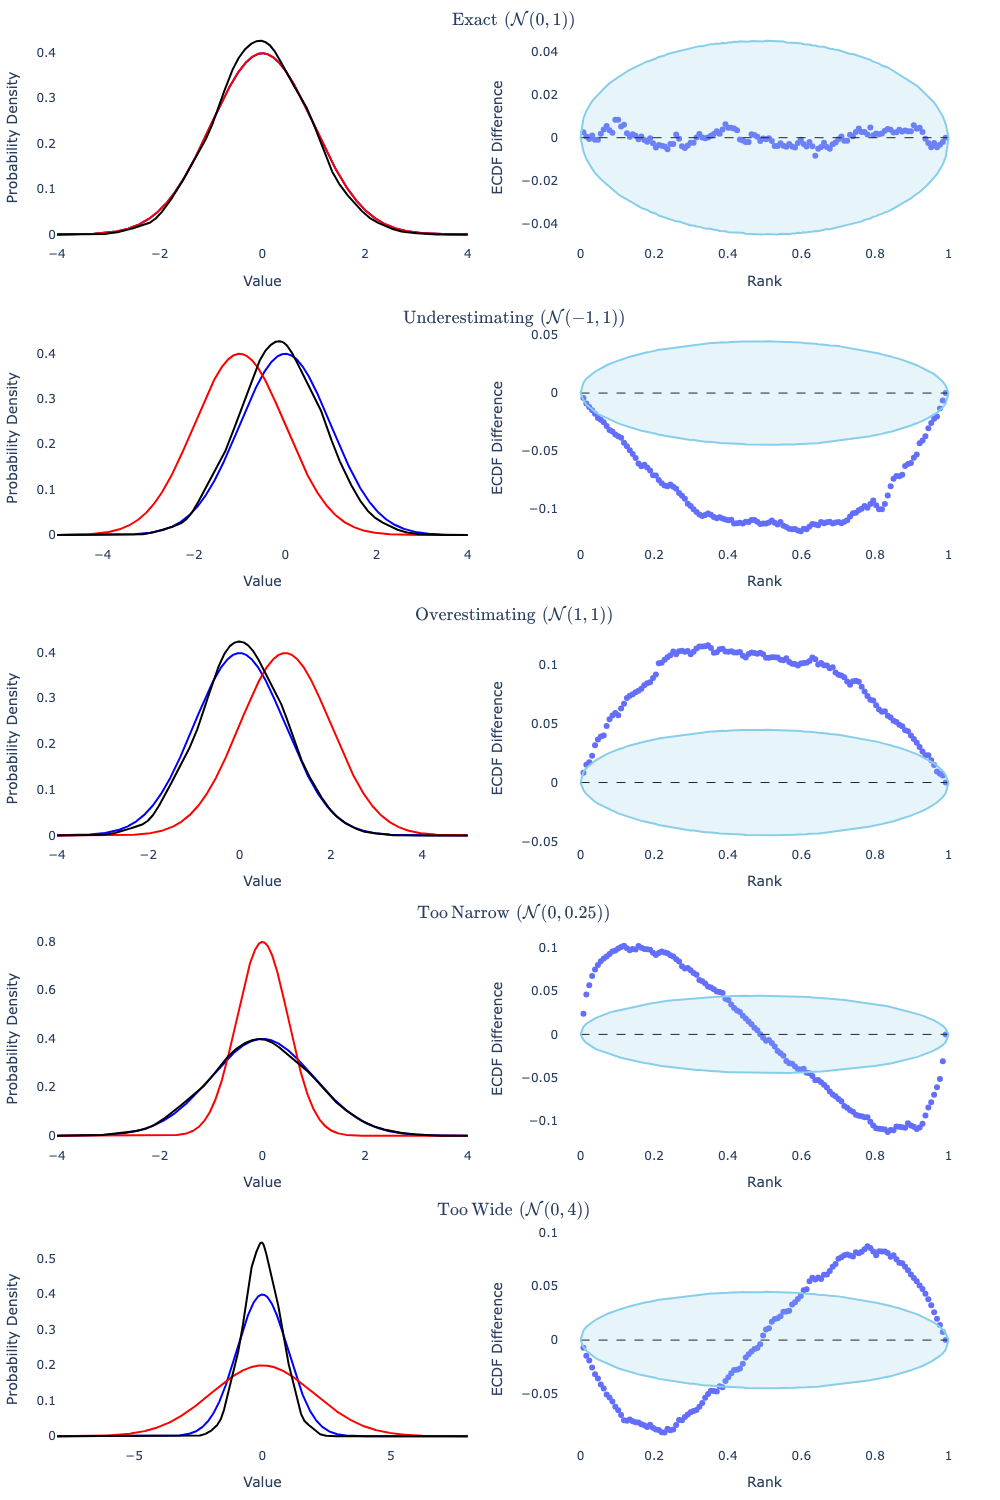
\includegraphics[width=0.85\linewidth]{figures/sbc_visualization.png}
    \caption{
        \textbf{SBC applied on synthetic data}.
        The true $\mu$ distribution is given by the blue distribution.
        The red distribution was set as data conditional distribution on inference process during the SBC validation.
        The black distribution is the kernel density estimate (KDE) for the $\mu$ posterior.
        The second column shows the ECDF difference plot for the normalized rank distribution.
        Under a well calibrated model, this ECDF is expected to be a straight line from $(0, 0)$ to $(1, 0)$.
    }
    \label{fig:sbc_viz}
\end{figure}

As we can see in Figure \ref{fig:sbc_viz}, a bias in the posterior reflects on a U-shape or an inverted U-shape in the ECDF differences plot.
On the other hand, under/overdispersion in the posterior results in a S-shape.
